\graphicspath{ {images/} }

\titledquestion{Attention Exploration}[14]
\label{sec:analysis}

Multi-head self-attention is the core modeling component of Transformers.
In this question, we'll get some practice working with the self-attention equations, and motivate why multi-headed self-attention can be preferable to single-headed self-attention.

Recall that attention can be viewed as an operation on a \textit{query} vector $q\in\mathbb{R}^d$, a set of \textit{value} vectors $\{v_1,\dots,v_n\}, v_i\in\mathbb{R}^d$, and a set of \textit{key} vectors $\{k_1,\dots,k_n\}, k_i \in \mathbb{R}^d$, specified as follows:
\begin{align}
&c = \sum_{i=1}^{n} v_i \alpha_i \\
&\alpha_i = \frac{\exp(k_i^\top q)}{\sum_{j=1}^{n} \exp(k_j^\top q)}
\end{align} 
with $alpha = \{\alpha_1, \ldots, \alpha_n\}$ termed the ``attention weights''. 
Observe that the output $c\in\mathbb{R}^d$ is an average over the value vectors weighted with respect to $\alpha$.

\begin{parts}

\part[3] \label{copying} \textbf{Copying in attention.} One advantage of attention is that it's particularly easy to ``copy'' a value vector to the output $c$. In this problem, we'll motivate why this is the case.

\begin{subparts}
    \subpart[2] The distribution $\alpha$ is typically relatively ``diffuse''; the probability mass is spread out between many different $\alpha_i$. However, this is not always the case. \textbf{Describe} (in one sentence) under what conditions the categorical distribution $\alpha$ puts almost all of its weight on some $\alpha_j$, where $j \in \{1, \ldots, n\}$ (i.e. $\alpha_j \gg \sum_{i \neq j} \alpha_i$). What must be true about the query $q$ and/or the keys $\{k_1,\dots,k_n\}$?

    \ifans{
        \newline
        The query $q$ must be very similar to the key $k_j$, such that $k_j^\top q \gg k_i^\top q$ for all $i \neq j$.
    }

    \subpart[1] Under the conditions you gave in (i), \textbf{describe} the output $c$. 

    \ifans{
        \newline
        $$
        c = \sum_{i=1}^{n} v_i \alpha_i \approx v_j \cdot 1 = v_j
        $$
    }

\end{subparts}


\part[2]\textbf{An average of two.} 
\label{q_avg_of_two}
Instead of focusing on just one vector $v_j$, a Transformer model might want to incorporate information from \textit{multiple} source vectors.

Consider the case where we instead want to incorporate information from \textbf{two} vectors $v_a$ and $v_b$, with corresponding key vectors $k_a$ and $k_b$.
Assume that (1) all key vectors are orthogonal, so $k_i^\top k_j = 0$ for all $i \neq j$; and (2) all key vectors have norm $1$.
\textbf{Find an expression} for a query vector $q$ such that $c \approx \frac{1}{2}(v_a + v_b)$, and \textbf{justify your answer}.\footnote{Hint: while the softmax function will never \textit{exactly} average the two vectors, you can get close by using a large scalar multiple in the expression.} (Recall what you learned in part~(\ref{copying}).)

\ifans{
    \newline
    Suppose that $q = \frac{k_a + k_b}{2}$, then we have:
    \begin{align*}
        \alpha_a &= \frac{\exp(k_a^\top q)}{\exp(k_a^\top q) + \exp(k_b^\top q)} \approx \frac{1}{2}\\
        \alpha_b &= \frac{\exp(k_b^\top q)}{\exp(k_a^\top q) + \exp(k_b^\top q)} \approx \frac{1}{2}\\
        c &= \sum_{i=1}^{n} v_i \alpha_i = v_a \cdot \alpha_a + v_b \cdot \alpha_b = \frac{1}{2}(v_a + v_b)
    \end{align*}
}

\part[5]\textbf{Drawbacks of single-headed attention:} \label{q_problem_with_single_head}
In the previous part, we saw how it was \textit{possible} for a single-headed attention to focus equally on two values.
The same concept could easily be extended to any subset of values.
In this question we'll see why it's not a \textit{practical} solution.

Consider a set of key vectors $\{k_1,\dots,k_n\}$ that are now randomly sampled, $k_i\sim \mathcal{N}(\mu_i, \Sigma_i)$, where the means $\mu_i \in \mathbb{R}^d$ are known to you, but the covariances $\Sigma_i$ are unknown (unless specified otherwise in the question).
Further, assume that the means $\mu_i$ are all perpendicular; $\mu_i^\top \mu_j = 0$ if $i\not=j$, and unit norm, $\|\mu_i\|=1$.

\begin{subparts}
\subpart[2] Assume that the covariance matrices are $\Sigma_i = \alpha I, \forall i \in \{1, 2, \ldots, n\}$, for vanishingly small $\alpha$.
Design a query $q$ in terms of the $\mu_i$ such that as before, $c\approx \frac{1}{2}(v_a + v_b)$, and provide a brief argument as to why it works.

\ifans{
    \newline
    Given that covariance matrices are $\Sigma_i = \alpha I, \forall i \in \{1, 2, \ldots, n\}$, for vanishingly small $\alpha$, we can approximate the key vectors as $k_i \approx \mu_i$.
    Suppose that $q = \frac{\mu_a + \mu_b}{2}$, then we have:
    \begin{align*}
        \alpha_a &= \frac{\exp(k_a^\top q)}{\exp(k_a^\top q) + \exp(k_b^\top q)} \approx \frac{1}{2}\\
        \alpha_b &= \frac{\exp(k_b^\top q)}{\exp(k_a^\top q) + \exp(k_b^\top q)} \approx \frac{1}{2}\\
        c &= \sum_{i=1}^{n} v_i \alpha_i = v_a \cdot \alpha_a + v_b \cdot \alpha_b = \frac{1}{2}(v_a + v_b)
    \end{align*}

}

\subpart[3] Though single-headed attention is resistant to small perturbations in the keys, some types of larger perturbations may pose a bigger issue. In some cases, one key vector $k_a$ may be larger or smaller in norm than the others, while still pointing in the same direction as $\mu_a$.\footnote{Unlike the original Transformer, newer Transformer models apply layer normalization before attention. In these pre-layernorm models, norms of keys cannot be too different which makes the situation in this question less likely to occur.}

As an example, let us consider a covariance for item $a$ as $\Sigma_a = \alpha I + \frac{1}{2}(\mu_a\mu_a^\top)$ for vanishingly small $\alpha$ (as shown in figure \ref{ka_plausible}). This causes $k_a$ to point in roughly the same direction as $\mu_a$, but with large variances in magnitude. Further, let $\Sigma_i = \alpha I$ for all $i \neq a$.
\begin{figure}[h]
\centering
\captionsetup{justification=centering,margin=2cm}
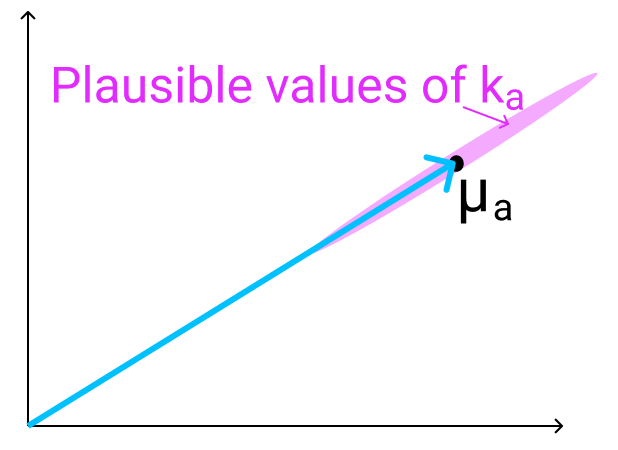
\includegraphics[width=0.35\linewidth]{images/ka_plausible.png}
\caption{The vector $\mu_a$ (shown here in 2D as an example), with the range of possible values of $k_a$ shown in red. As mentioned previously, $k_a$ points in roughly the same direction as $\mu_a$, but may have larger or smaller magnitude.}
\label{ka_plausible}
\end{figure}

When you sample $\{k_1,\dots,k_n\}$ multiple times, and use the $q$ vector that you defined in part i., what do you expect the vector $c$ will look like qualitatively for different samples? Think about how it differs from part (i) and how $c$'s variance would be affected.

\ifans{
    \newline
    In part (ii), the key $k_a$ has large variance along the direction of $\mu_a$. We can model this as $k_a \approx \lambda \mu_a$, where $\lambda$ is a scalar with large variance.

    Using the same query $q = \frac{\mu_a + \mu_b}{2}$, the dot products become:
    \begin{align*}
    k_a^T q &\approx (\lambda \mu_a)^T \left(\frac{\mu_a + \mu_b}{2}\right) = \frac{\lambda}{2} (\mu_a^T \mu_a + \mu_a^T \mu_b) = \frac{\lambda}{2} \\
    k_b^T q &\approx \mu_b^T \left(\frac{\mu_a + \mu_b}{2}\right) = \frac{1}{2} (\mu_b^T \mu_a + \mu_b^T \mu_b) = \frac{1}{2}
    \end{align*}
    The inputs to the softmax are now $(\lambda/2, 1/2)$. Since $\lambda$ has high variance, the attention weights $\alpha_a$ and $\alpha_b$ become unstable.
    \begin{itemize}
        \item If $\lambda \gg 1$, then $\alpha_a \approx 1$ and $\alpha_b \approx 0$.
        \item If $\lambda \ll 1$, then $\alpha_a \approx 0$ and $\alpha_b \approx 1$.
    \end{itemize}
    Consequently, the context vector $c = \alpha_a v_a + \alpha_b v_b$ will randomly jump between $v_a$ and $v_b$ across different samples.
    This means the variance of $c$ will be large, making the attention output unstable and difficult to learn from.
}
\end{subparts}

\part[3]\textbf{Benefits of multi-headed attention:} \label{q_multi_head}
Now we'll see some of the power of multi-headed attention.
We'll consider a simple version of multi-headed attention which is identical to single-headed self-attention as we've presented it, except two query vectors ($q_1$ and $q_2$) are defined, which leads to a pair of vectors ($c_1$ and $c_2$), each the output of single-headed attention given its respective query vector.
The final output of the multi-headed attention is their average, $\frac{1}{2}(c_1+c_2)$.

As in question 1(\ref{q_problem_with_single_head}), consider a set of key vectors $\{k_1,\dots,k_n\}$ that are randomly sampled, $k_i\sim \mathcal{N}(\mu_i, \Sigma_i)$, where the means $\mu_i$ are known to you, but the covariances $\Sigma_i$ are unknown.
Also as before, assume that the means $\mu_i$ are mutually orthogonal; $\mu_i^\top \mu_j = 0$ if $i\not=j$, and unit norm, $\|\mu_i\|=1$.

\begin{subparts}
\subpart[1]
Assume that the covariance matrices are $\Sigma_i=\alpha I$, for vanishingly small $\alpha$.
Design $q_1$ and $q_2$ in terms of $\mu_i$ such that $c$ is approximately equal to $\frac{1}{2}(v_a+v_b)$. 
Note that $q_1$ and $q_2$ should have different expressions.

\ifans{
    \newline
    We can design the query vectors as follows:
    \begin{align*}
        &q_1 = \mu_a, q_2 = \mu_b\\
        &c_1 = q_1 = v_a, c_2 = q_2 = v_b\\
        &c = \frac{1}{2}(c_1 + c_2) = \frac{1}{2}(v_a + v_b)
    \end{align*}

}

\subpart[2]
Assume that the covariance matrices are $\Sigma_a=\alpha I + \frac{1}{2}(\mu_a\mu_a^\top)$ for vanishingly small $\alpha$, and $\Sigma_i=\alpha I$  for all $i \neq a$.
Take the query vectors $q_1$ and $q_2$ that you designed in part i.
What, qualitatively, do you expect the output $c$ to look like across different samples of the key vectors? Explain briefly in terms of variance in $c_1$ and $c_2$. You can ignore cases in which $k_a^\top q_i < 0$.

\ifans{
    \newline
    Using the same query vectors $q_1 = \mu_a$ and $q_2 = \mu_b$, we have:
    \begin{align*}
        &k_a = \lambda \mu_a, \text{ where } \lambda \text{ has high variance.}\\
        &k_b \approx \mu_b\\
        &k_a^\top q_1 \approx \lambda, k_b^\top q_1 = 0\\
        &c_1 = v_a, c_2 = v_b\\
        &c = \frac{1}{2}(c_1 + c_2) = \frac{1}{2}(v_a + v_b)
    \end{align*}
}
\end{subparts}

\part[1] Based on part~(\ref{q_multi_head}), briefly summarize how multi-headed attention overcomes the drawbacks of single-headed attention that you identified in part~(\ref{q_problem_with_single_head}).

\ifans{
    Multi-headed attention overcomes this by allowing different heads to "divide the labor" and specialize. In part (d), one head specialized in finding $k_a$ and the other in finding $k_b$. The variance in $k_a$'s magnitude only affected the first head, while the second head, focused on $k_b$, was completely isolated from this noise. By combining the stable outputs from these independent and specialized heads, the final output remains robust and low-variance, effectively ignoring the noise that crippled the single-headed system.
}

\end{parts}
